%!TEX root = bipartite.tex

\section{Related Work} \label{sec:related}

\iffalse
\begin{figure}[t]
\centering
  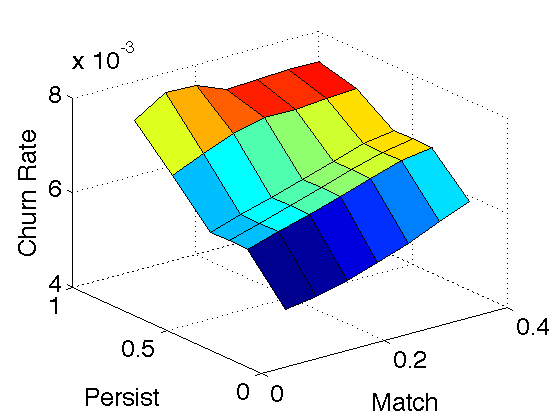
\includegraphics[width=8cm]{./figures/persist-parameters.png}  
  \caption{Typical figure.}  
\label{fig:typical}
\end{figure}
\fi

Then the community membership of the churners for months five and six were examined - see Table \ref{tab:rate1} and also Figure \ref{fig:typical}. The most striking thing to note is that the churn rate among unassigned nodes is an order of magnitude lower than that of nodes assigned to communities. 
Note that, while the MOSES algorithm will often assign nodes to multiple communities, it can also leave some nodes ``unassigned'' (\ie not assigned to any community at all).


Then the community membership of the churners for months five and six were examined - see Table \ref{tab:rate1} and also Figure \ref{fig:typical}. The most striking thing to note is that the churn rate among unassigned nodes is an order of magnitude lower than that of nodes assigned to communities. 
Note that, while the MOSES algorithm will often assign nodes to multiple communities, it can also leave some nodes ``unassigned'' (\ie not assigned to any community at all).

\begin{table}[!h]
\centering
\begin{tabular}{ l c | c c c c } 
Month \;\; & Churn rate & Churn rate assigned & Churn Rate unassigned \\
\hline 
1 & 0.42\% & 0.524\% & 0.050\% \\ 
2 & 0.43\% & 0.533\% & 0.053\%  \\ 
3 & 0.43\% & 0.534\% & 0.049\%  \\ 
4 & 0.44\% &  0.546\%  & 0.055\% \\
Aggregated & 0.36\% &  0.441\%  & 0.015\%  \\
\end{tabular}
\caption{Churn rate for assigned and unassigned nodes in the communities identified by the MOSES algorithm on the monthly call graphs, and on the aggregated four month graph.}
\label{tab:rate1}
\end{table}